\newcommand{\ggfusion}{
\begin{fmffile}{ggfusion} 	%one.mf will be created for this feynman diagram  
\fmfframe(1,7)(1,7){ 	%Sets dimension of Diagram
\begin{fmfgraph*}(110,102) %Sets size of Diagram
\fmftop{g1,g1p}
\fmfbottom{g2,g2p}
\fmfright{H}    %Sets there to be 2  outputs
%\fmflabel{$g$}{g1}
%\fmflabel{$g$}{g2}
\fmflabel{$H$}{H}
\fmf{gluon,lab=$g$,lab.sid=left}{g1,v1} %Connects the sources with a vertex.
\fmf{gluon,lab=$g$,lab.sid=left}{g2,v2} %Connects the sources with a vertex.
\fmf{phantom}{v1,g1p}
\fmf{phantom}{v2,g2p}
\fmf{fermion,tension=.4}{v1,v2,v3,v1} %Connects the sources with a vertex.
\fmf{dashes}{H,v3}
\end{fmfgraph*}
}
\end{fmffile}
}

\section{History of Higgs Searches}
\label{sec:history}
The Higgs boson is arguably the most outstanding piece of the SM, and as such it has been the topic of intense study.
Two experiments that have previously searched for the Higgs boson are the Large Electron-Positron Collider (LEP), and the Tevatron.
\subsection{The Standard Model Higgs Search}
The dominant production mechanism at LEP  was the Higgstrahlung process, this was also the most relevant process at the Tevatron. 
The Higgstrahlung process proceeds by producing a gauge boson in either an electron/positron collision (LEP) or quark/anti-quark collision (Tevatron), the gauge boson then radiates a Higgs boson.
The Feynman diagram for this process is shown in Figure \ref{fig:higgstrahlung}
\begin{figure}[htpb]
\begin{center}
\begin{fmffile}{higgstrahlung} 	%one.mf will be created for this feynman diagram  
\fmfframe(1,7)(1,7){ 	%Sets dimension of Diagram
\begin{fmfgraph*}(110,62) %Sets size of Diagram
\fmfleft{q1,q2}
\fmflabel{$q,e^{-}$}{q1}
\fmflabel{$\overline{q},e^{+}$}{q2}
\fmflabel{$H$}{H}
\fmfright{V,H}    %Sets there to be 2  outputs
\fmflabel{$Z$}{V}
\fmf{fermion}{q1,v1,q2} %Connects the sources with a vertex.
\fmf{photon,label=$Z^{*}$}{v1,v2}
\fmf{photon}{v2,V}
\fmf{dashes}{v2,H}
\end{fmfgraph*}
}
\end{fmffile}
\caption{Feynman diagram of the Higgstrahlung process, with incoming  $e^{+}e^{-}$ as at LEP or $q\overline{q}$ as would be seen at the Tevatron.}
\label{fig:higgstrahlung}
\end{center}
\end{figure}

LEP was an $e^{+}e^{-}$ collider located at CERN and has excluded the presence of a standard model Higgs boson with mass less than $114$ GeV.
LEP performed a search for the Higgs boson over several search channels, the majority of which include the Higgs decaying to two bottom quarks and the Z decaying to a number of different states including: $q\overline{q}$, $t\overline{t}$, $\nu\overline{\nu}$, $\mu^{+}\mu^{-}$, and $e^{+}e^{-}$\cite{PDGREVIEW}.
The combined LEP Higgs boson exclusion can be seen in Figure \ref{fig:lepexclusion}.
\begin{figure}[htpb]
\begin{center}
\centerline{\includegraphics[width=0.85\textwidth]{plots/lephiggs.png}}%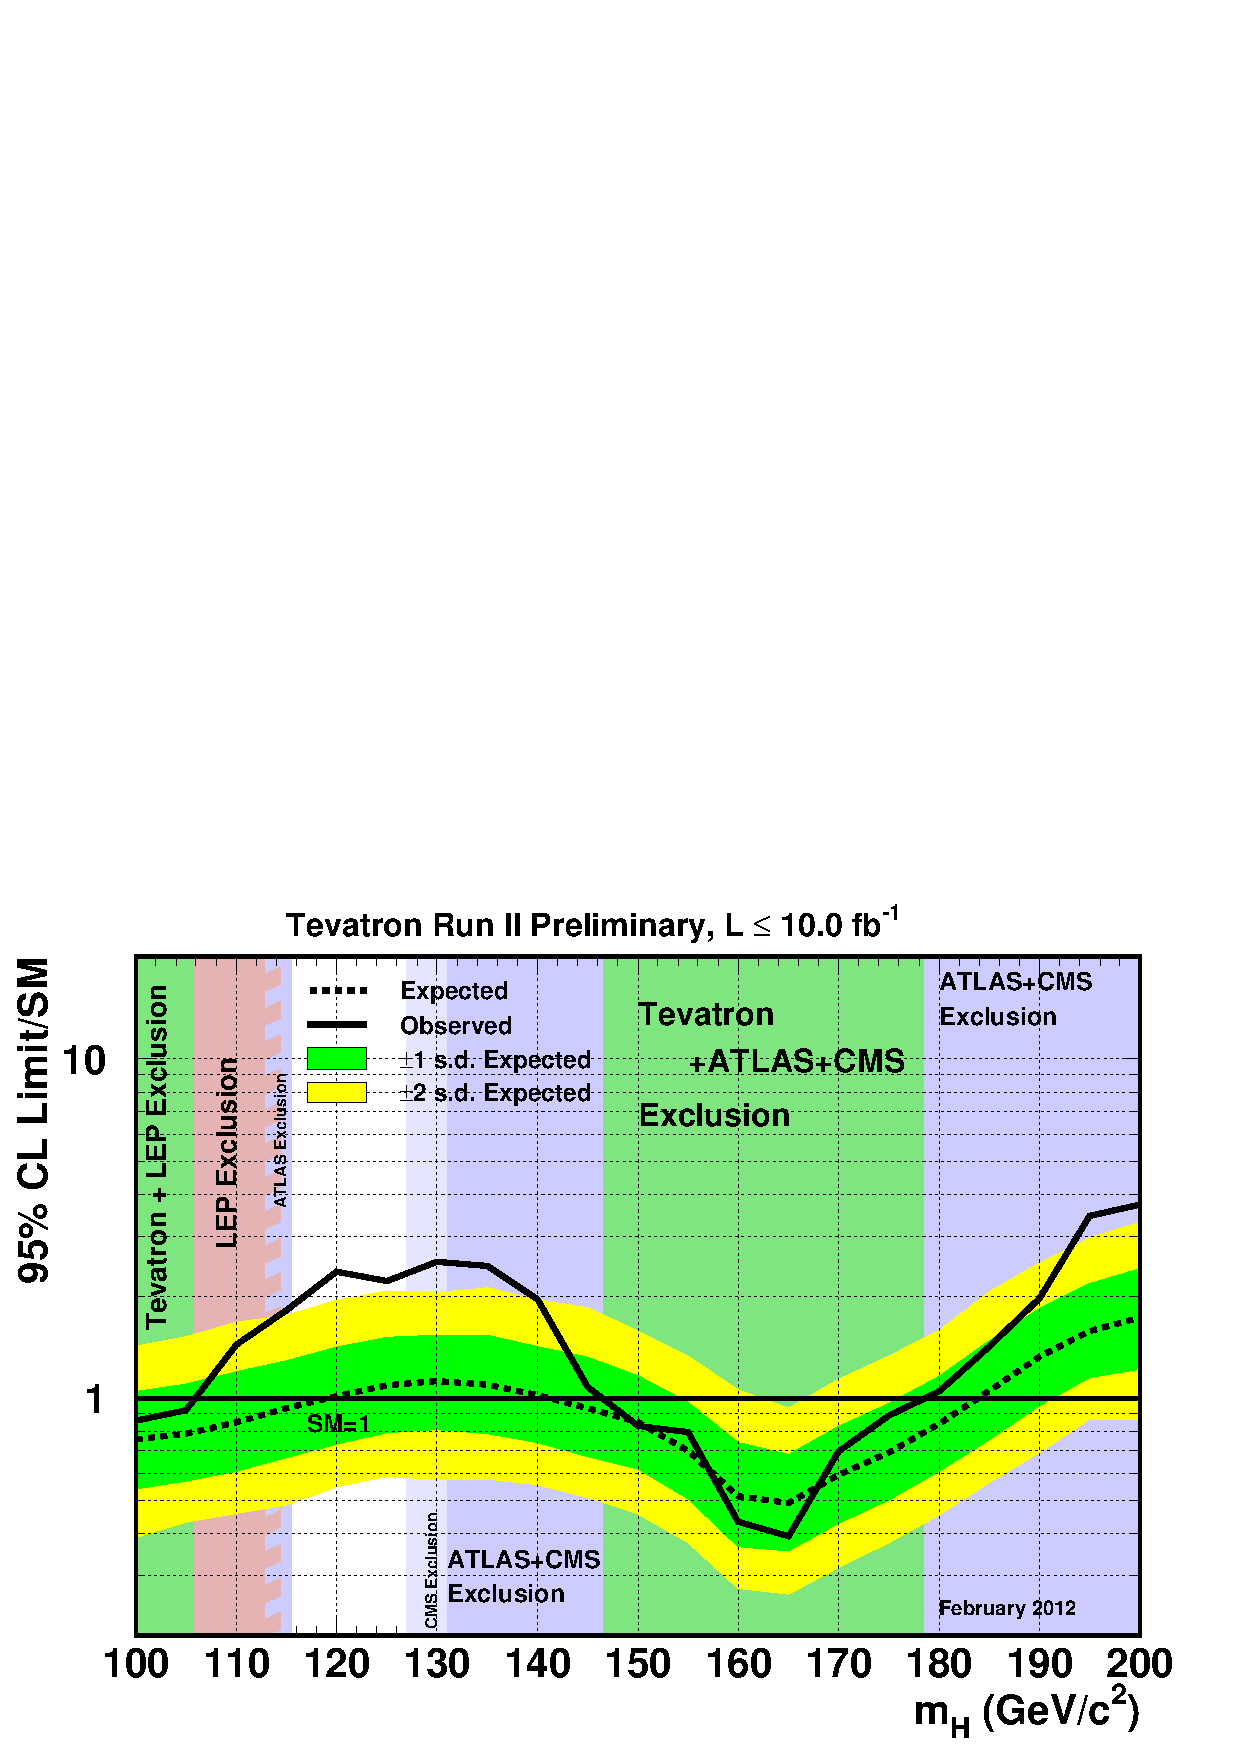
\includegraphics[width=0.4\textwidth]{plots/tev28febsmbayeslimits.pdf}}
%\centerline{\includegraphics[width=0.4\textwidth]{plots/cmshiggs.pdf}\includegraphics[width=0.4\textwidth]{plots/atlashiggs.pdf}}
\caption{
  Higgs exclusion as a function of mass at LEP\cite{PDGREVIEW}.
}
\label{fig:lepexclusion}
\end{center}
\end{figure}

The Tevatron was a $p\overline{p}$ collider located at Fermilab National Laboratory, just west of Chicago, IL. 
It operated at a center of mass energy $\sqrt{s} = 1.96$ TeV.
At the Tevatron a number of different channels contributed to the sensitivity of the Higgs search, the more notable being $H \rightarrow b\overline{b}$ at low Higgs mass, and $H \rightarrow W^{+}W^{-}$ at higher mass\cite{TEVHIGGS}.
The combined Tevatron Higgs exclusion can be seen in Figure \ref{fig:tevexclusion}.
The Tevatron has two exclusion regions, the first is $100 < m_{H} < 106$ GeV, and the second being $147 < m_{H} < 179$ GeV.
Further, the result contains an excess of events above background expectations in the range $115 < m_{H} < 135$ GeV with a global significance of approximately 2.2 standard deviations.
\begin{figure}[htpb]
\centerline{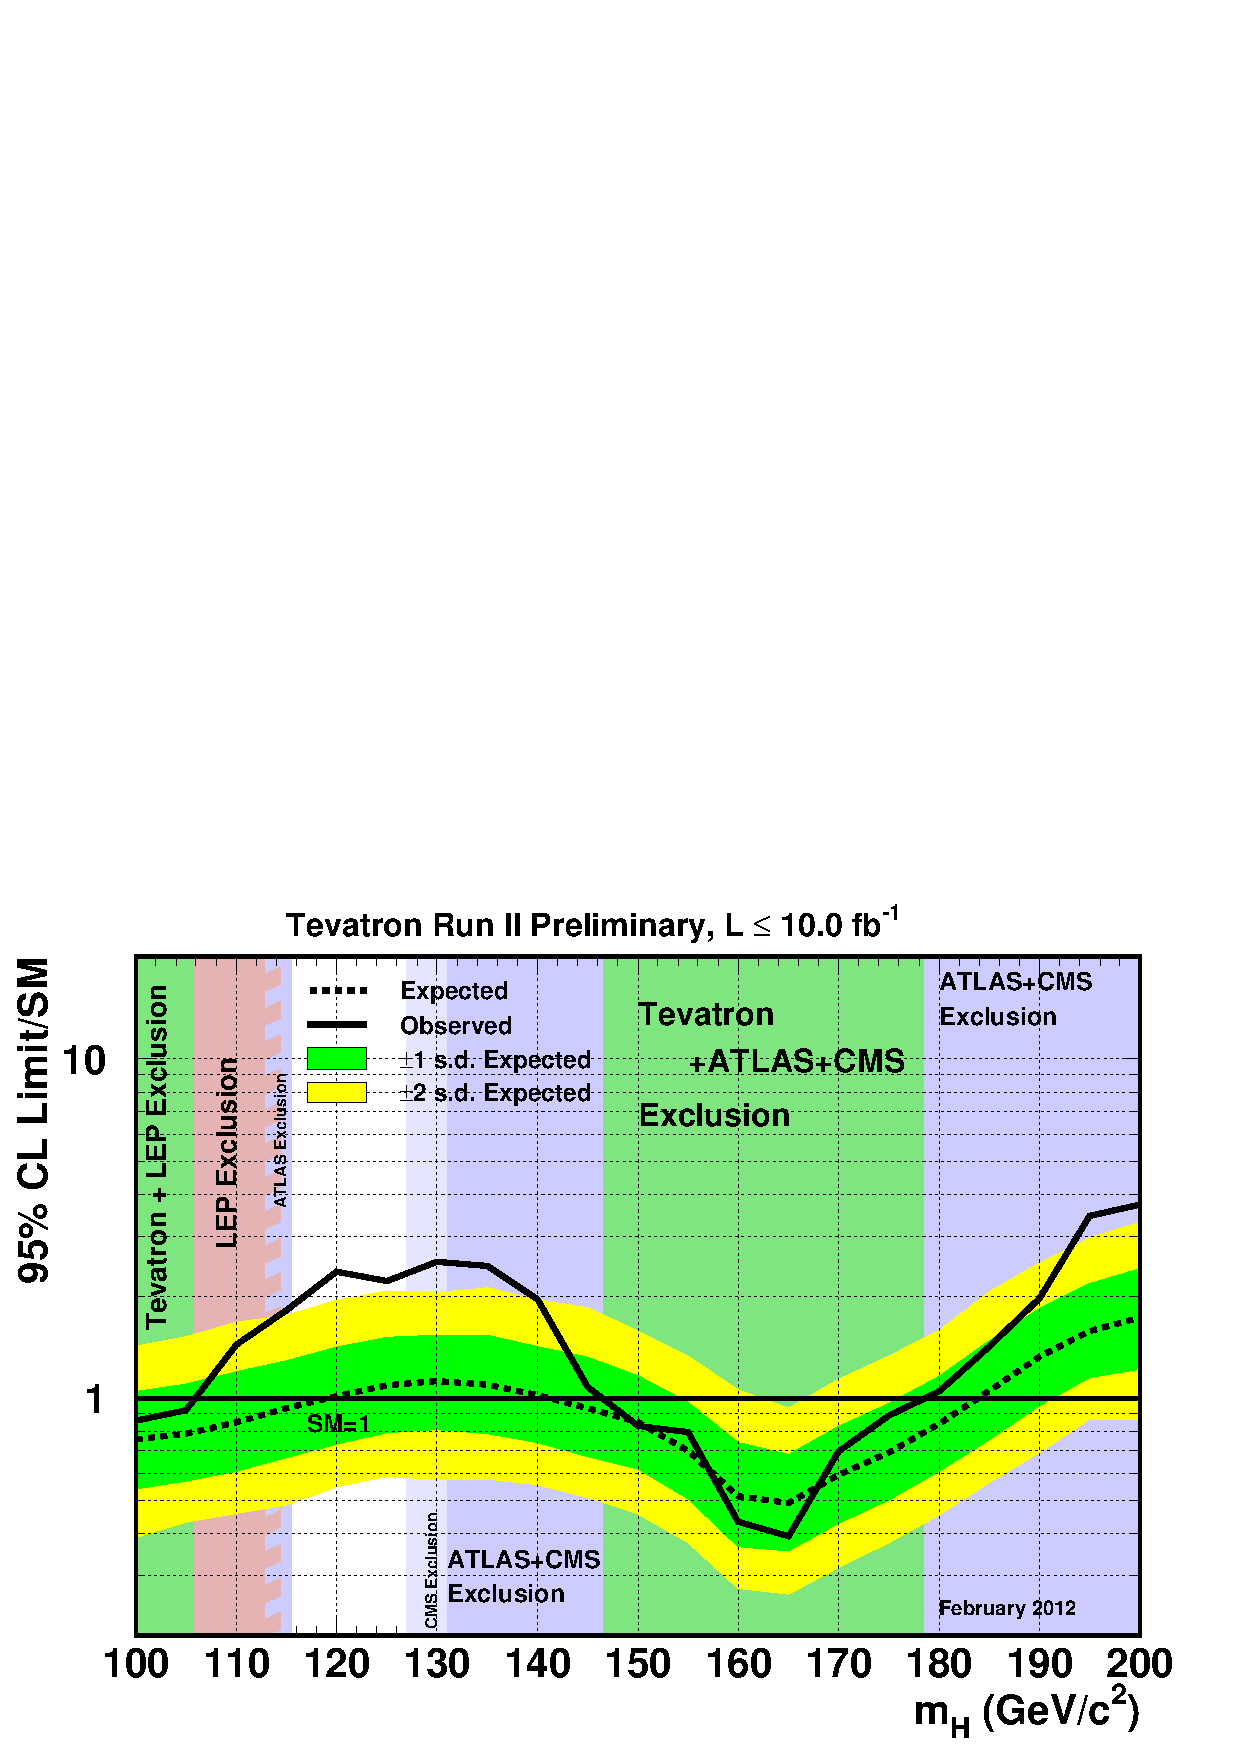
\includegraphics[width=0.85\textwidth]{plots/tev28febsmbayeslimits.pdf}}
\caption{Higgs exclusion at Tevatron\cite{TEVHIGGS}.}
\label{fig:tevexclusion}
\end{figure}

Due to the higher momentum protons at the LHC, it is much more probable that two gluons will interact to produce a Higgs boson, thus the dominant production mechanism is gluon gluon fusion.
Gluon gluon fusion is the process by which two gluons produce a Higgs boson through a fermion loop, shown in the left hand side of Figure \ref{fig:smproduction}\cite{PDGREVIEW}. 
A smaller, but still significant production mechanism at the LHC is vector boson fusion, as shown in the right hand side of Figure \ref{fig:smproduction}.
In vector boson fusion, two incoming quarks each radiate a gauge boson which then fuse, producing a Higgs boson.
The production cross sections as a function of the Higgs mass can be seen in the left hand side of Figure \ref{fig:higgsproduction}.
One can see that the production rate of vector boson fusion is approximately one tenth that of gluon fusion. 
Due to the lack of color change in this process it yields the unique signature of having low central jet activity while having two boosted jets in either hemisphere of the detector.
This unique signature makes it possible to identify and remove events of many background processes that would otherwise make the measurement more difficult.
\begin{figure}
\begin{center}
\ggfusion
\begin{fmffile}{vectorbosonfusion} 	%one.mf will be created for this feynman diagram  
\fmfframe(0,10)(0,10){ 	%Sets dimension of Diagram
\begin{fmfgraph*}(110,102) %Sets size of Diagram
\fmftop{iq1,oq1}
\fmfbottom{iq2,oq2}
\fmfright{H}    %Sets there to be 2  outputs
\fmflabel{$q$}{iq1}
\fmflabel{$q$}{oq1}
\fmflabel{$q^{\prime}$}{iq2}
\fmflabel{$q^{\prime}$}{oq2}
\fmflabel{$H$}{H}
\fmf{fermion,tension=2}{iq1,v1,oq1} %Connects the sources with a vertex.
\fmf{fermion,tension=2}{iq2,v2,oq2} %Connects the sources with a vertex.
\fmf{photon,label=$W^{\pm}/Z$}{v1,v3}
\fmf{photon,label=$W^{\mp}/Z$}{v2,v3}
\fmf{dashes,tension=.1}{H,v3}
\end{fmfgraph*}
}
\end{fmffile}
\caption{
  Feynman diagrams of prominent SM Higgs production mechanisms at the LHC. Gluon fusion (left) and vector boson fusion (right).
}
\label{fig:smproduction}
\end{center}
\end{figure}

Both the Compact Muon Solenoid (CMS) and A Large Toroidal LHC Apparatus (ATLAS) have performed Higgs searches in a broad number of channels.
One can see from Figure \ref{fig:higgsproduction} that in the low Higgs mass regime the branching ratio of $H\rightarrow b\overline{b}$ dominates, however due to the high cross section of QCD multi-jet events this is a very difficult channel at the LHC.
Rather than $H \rightarrow b\overline{b}$ contributing most to the sensitivity at low Higgs mass, it is in the $H\rightarrow\gamma\gamma$ channel that the majority of the sensitivity lies.
The sensitivity of the $H\rightarrow\gamma\gamma$ channel is due primarily to the low number of background processes that are associated with it.
In the high mass region as the branching ratios indicate, the $H\rightarrow WW$ and $H\rightarrow ZZ$ channels are the dominant search channels.
The combined Higgs exclusion for the CMS detector can be seen in Figure \ref{fig:lhcexclusion}.
Between CMS and ATLAS the exclusion range for the Higgs is found to be $127 < m_{H} < 600$ GeV.
Both experiments see a similar excess in the region around $124$ GeV, CMS with a local significance of $3.1\sigma$ and a global significance of $2.1\sigma$.
With more than one indication of an excess of signal, it is an exciting time in High Energy Physics as a breakthrough may be right around the corner.
\begin{figure}[htpb]
\begin{center}
%\includegraphics[width=0.4\textwidth]{plots/tevhiggsproduction.png}
\centerline{\includegraphics[width=0.51\textwidth]{plots/lhchiggsproduction.png}\includegraphics[width=0.38\textwidth]{plots/higgsbr.jpg}}
\caption{Standard Model Higgs boson production cross sections at the LHC energy scale\cite{HIGGS_PRODUCTION}.}
\label{fig:higgsproduction}
\end{center}
\end{figure}

\begin{figure}[htpb]
\label{fig:lhcexclusion}
\begin{center}
\centerline{\includegraphics[width=0.60\textwidth]{plots/cmshiggs.pdf}}
%\centerline{\includegraphics[width=0.63\textwidth]{plots/atlashiggs.pdf}}
\caption{Higgs exclusion as a function of mass at CMS\cite{CMSHIGGS}.}
\label{fig:lhcexclusion}
\end{center}
\end{figure}

\subsection{The Higgs Search in the Minimal Supersymmetric Standard Model}
If the excess of signal seen at the Tevatron and the LHC does indeed yield a discovery of the Higgs boson at a mass around $124$ GeV, it does not signify the end of the story for the Higgs boson.
As discussed in Section \ref{sec:mssm}, the MSSM will likely induce an enhanced coupling between the Higgs boson and bottom quarks and tau leptons as per Equation \ref{eqn:mssmcouplings}.
Indeed at a mass of $124$ GeV, this puts the Higgs at a mass in which the branching ratio to tau leptons is favorable, and in the case of the MSSM the Higgs will decay to tau leptons approximately $10\%$ of the time, and to bottom quarks approximately $90\%$ of the time.
The difficulty in performing an analysis involving bottom quarks in a hadron collider environment such as the LHC makes the search for the Higgs in the channel $H\rightarrow\tau^{+}\tau^{-}$ all the more attractive.

In the MSSM, the dominant Higgs production mechanisms are slightly different than the SM.
In particular, the cross section and branching ratio to tau leptons for the heavy CP-even ($H$) and CP-odd ($A^{0}$) Higgs bosons are considered.
While the gluon fusion production mechanism remains dominant as in the SM, due to the enhanced coupling to the bottom quark the vector boson fusion mechanism is supplanted by the associated production with bottom quarks as shown in the right hand side of Figure \ref{fig:mssmproduction}.
Not only does the associated production mechanism rate increase, but at high $tan\beta$ this mechanism can have a greater cross section than that of gluon fusion.
The production cross section times branching ratio to two tau leptons ($\sigma\times BR(\tau\tau)$) for the MSSM as compared to the SM can be seen in the left portion of Figure \ref{fig:mssmcrosssections}, while the enhanced branching ratio to the tau lepton can be seen on the right.
One can see that the branching ratio to tau leptons remains constant over a much larger mass range than in the SM.
This enhancement comes at the expense of a decreased branching ratio to $W$ and $Z$ bosons, making the search in the $H\rightarrow\tau\tau$ channel very important.
\begin{figure}
\begin{center}
\ggfusion
\begin{fmffile}{associatedprod} 	%one.mf will be created for this feynman diagram  
\fmfframe(1,7)(1,7){ 	%Sets dimension of Diagram
\begin{fmfgraph*}(110,102) %Sets size of Diagram
\fmftop{g1,b1}
\fmfbottom{g2,b2}
\fmfright{H}    %Sets there to be 2  outputs
\fmflabel{$g$}{g1}
\fmflabel{$g$}{g2}
\fmflabel{$H$}{H}
\fmflabel{$b$}{b2}
\fmflabel{$\overline{b}$}{b1}
\fmf{gluon,tension=2}{g1,v1} %Connects the sources with a vertex.
\fmf{gluon,tension=2}{g2,v2} %Connects the sources with a vertex.
\fmf{fermion,tension=2}{b1,v1,v3,v2,b2} %Connects the sources with a vertex.
\fmf{dashes,tension=.1}{H,v3}
\end{fmfgraph*}
}
\end{fmffile}
\caption{
  Feynman diagrams of prominent MSSM Higgs production mechanisms at the LHC. Gluon fusion (left) and associated production with b quarks (right).
}
\label{fig:mssmproduction}
\end{center}
\end{figure}
\begin{figure}[htpb]
\begin{center}
\centerline{\includegraphics[width=0.45\textwidth]{plots/cross-sections.pdf}\includegraphics[width=0.45\textwidth]{plots/branching-ratios.pdf}}
\caption{
  On the left the Higgs production cross sections are compared between MSSM and SM mechanisms. The blue and red bands represent the range of the cross section between low $tan\beta = 5$ and high $tan\beta = 30$. On the right the branching ratio for $H\rightarrow\tau^{+}\tau^{-}$ is compared for various values of $tan\beta$ in the MSSM to the SM branching ratio}
\label{fig:mssmcrosssections}
\end{center}
\end{figure}

